	
	\subsection*{1.}
	
	\subsubsection*{a.}
	
\begin{center}
	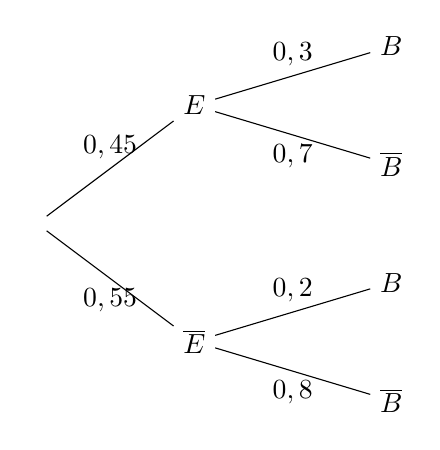
\begin{tikzpicture}
		[level 1/.style={level distance=2cm,
			sibling distance=3cm},
		level 2/.style={level distance=2.5cm,
			sibling distance=1.5cm}]
		\node {} [grow'=right]
		child {node {$E$}
			child {node {$B$}
				edge from parent node[above] {$0,3$}
			}
			child {node {$\overline B$}
				edge from parent node[below] {$0,7$}
			}
			edge from parent node[above] {$0,45$}
		}
		child {node {$\overline E$}
			child {node {$B$}
				edge from parent node[above] {$0,2$}
			}
			child {node {$\overline B$}
				edge from parent node[below] {$0,8$}
			}
			edge from parent node[below] {$0,55$}
		}
		;
	\end{tikzpicture}
\end{center}
	
	\subsubsection*{b.}
	
	\[
	\begin{aligned}
		P(E \cap B) &= P(E) \times P_E(B) = 0,45 \times 0,30 = 0,135, \\
		P(\overline{E} \cap B) &= P(\overline{E}) \times P_{\overline{E}}(B) = 0,55 \times 0,20 = 0,11.
	\end{aligned}
	\]
	
	D'après la loi des probabilités totales :
	\[
	P(B) = P(E \cap B) + P(\overline{E} \cap B) = 0,135 + 0,11 = 0,245.
	\]
	
	\subsubsection*{c.}
	
	On calcule
	$	P_B(E) = \dfrac{P(B \cap E)}{P(B)} = \dfrac{P(E \cap B)}{P(B)} = \dfrac{0,135}{0,245} \approx 0,55102 $\\
	\quad soit \quad 0,551 \quad au millième près.
	
	
	\subsection*{2.}
	
	\subsubsection*{a.}
	

	\[
	\begin{array}{|c|c|c|c|c|}
		\hline	x_i & 20 & 50 & 60 & 90 \\
		\hline
		P(X = x_i) & 0,44 & 0,315 & 0,11 & 0,135 \\
			\hline
	\end{array}
	\]
	
	\subsubsection*{b.}
	
	L'espérance mathématique de la variable aléatoire est égale à :
	\[
	E(X) = 20 \times 0,44 + 50 \times 0,315 + 60 \times 0,11 + 90 \times 0,135 = 8,8 + 15,75 + 6,6 + 12,15 = 45,30.
	\]
	
	Ceci représente le coût moyen de réparation par téléphone.
	
	Donc pour 500 téléphones, la dépense de l'entreprise sera environ de :
	\[
	500 \times 45,30 = 22 650 \, \text{euros}.
	\]
	
